\chapter{Wybór technologii oraz narzędzi}


\section{Wykrywanie twarzy na zdjęciu}

Wykrywanie twarzy to pierwszy krok w zaprojektowanym systemie.
Z powodu tego, że jest on umieszczony na samym początku, proces ten musi być maksymalnie skuteczny.
Jeżeli na zdjęciu nie zostanie wykryta twarz, to cały proces zakończy się z negatywnym rezultatem.
\textbf{Twarzy nie będzie można zidentyfikować, jeżeli nie zostanie ona znaleziona.}
Niestety twarz ludzka jest obiektem dynamicznym i ma duży stopień zmienności w wyglądzie,
co sprawia, że wykrywanie twarzy jest trudnym problemem w widzeniu komputerowym~\cite{HJELMAS2001236}.

W artykule z 2016 roku zatytułowanym
``Joint Face Detection and Alignment Using Multitask Cascaded Convolutional Networks''~\cite{zhang2016joint}
została zaproponowana wielozadaniowa kaskadowa konwolucyjna sieć neuronowa
(ang. Multi-Task Cascaded Convolutional Neural Networks - MTCNN) do wykrywania twarzy.
Sieć ta zyskała duża popularność, ponieważ osiągnęła wówczas najlepszy wyniki
w wykrywaniu twarzy na zdjęciach dla wybranych zbiorów danych.
Kolejną zaletą zaproponowanej sieci neuronowej jest to, że jest w stanie
rozpoznać punkty orientacyjne twarzy, takie jak oczy, usta i nos.

W internecie znajduje się spora liczba implementacji MTCNN~\cite{mtznn_all_impls}.
Spośród dostępnych została wybrana sieć napisana przez \textit{Iván de Paz Centeno}
i udostępniona na portalu GitHub\footnote{GitHub - dostawcą platformy internetowej do tworzenia
oprogramowania i kontroli wersji za pomocą narzędzia Git udostępniania
pod adresem \url{https://github.com}. } (\url{https://github.com/ipazc/mtcnn}) na zasadach licencji MIT\footnote{Licencja MIT daje użytkownikom
nieograniczone prawo do używania, kopiowania, modyfikowania i rozpowszechniania (w tym sprzedaży)
    oryginalnego lub zmodyfikowanego programu.
    Jedynym wymaganiem jest, by we wszystkich wersjach zachowano warunki licencyjne i informacje o autorze.
}~\cite{ipazc/mtcnn}.
Główną zaletą wybranej implementacji jest łatwość użycia.
Sieć została napisana w języku programowania python w bibliotece TensorFlow
i całość udostępniona jako pakiet z możliwością instalacji
przez PIP\footnote{PIP - narzędzie do instalowania pakietów python}.


\section{FaceNet}

FaceNet to architektura oparta na głębokiej sieci neuronowej, która bezpośrednio uczy się mapowania
z obrazów twarzy do n-wymiarowych wektorów, gdzie poszczególne wartości wektora charakteryzują daną twarz.
Wymiarowość wektora jest zależna od konkretnej implementacji.
W przestrzeni składającej się z wygenerowanych wektorów
odległości pomiędzy wektorami, mierzone za pomocą metryki euklidesowej,
bezpośrednio odpowiadają mierze podobieństwa twarzy.
Oznacza to, że zadania polegające na identyfikacji, weryfikacji czy grupowaniu
sprowadzają się do pomiaru odległości pomiędzy poszczególnymi wektorami cech~\cite{schroff2015facenet}.
Wizualizacja procesu mapowania zdjęcia do przestrzeni
euklidesowej została przedstawiona na rysunku~\ref{fig:facenet_zastosowanie}.

\begin{figure}[H]
    \centering
    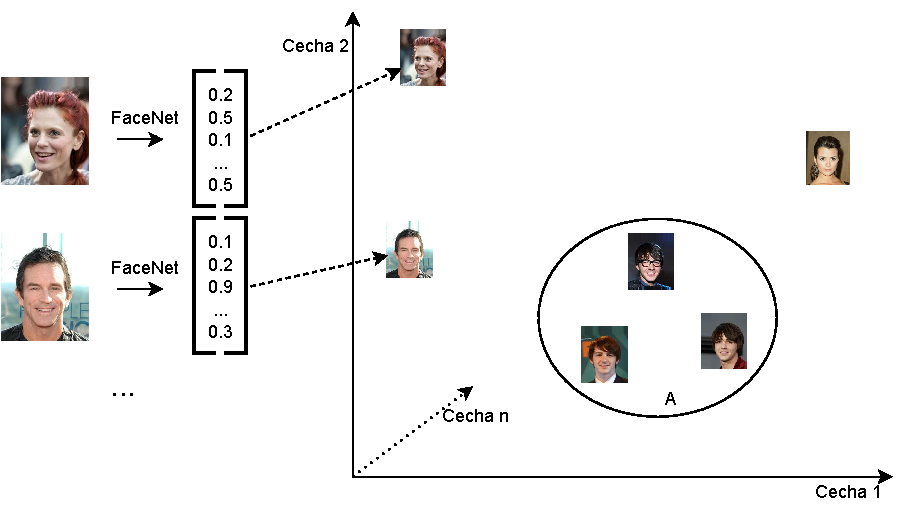
\includegraphics[width=.8\textwidth]{images/facenet_euc}
    \caption{
        Wizualizacja przestrzeni składającej się z wygenerowanych wektorów.
        Odległości mierzone metryką euklidesową pomiędzy wektorami reprezentującymi te
        same osoby są mniejsze względem wektorów reprezentujących inne osoby.
        Literą ``A'' zostały oznaczone zdjęcia przedstawiające tę samą osobę.
    }
    \customsource
    \label{fig:facenet_zastosowanie}
\end{figure}

\pagebreak

\subsection{Zasada działania}


Po dostarczeniu danego zdjęcia do sieci następuje wieloetapowa filtracja przy użyciu filtrów splotowych,
aby wydobyć z obrazu na wejściu wyróżniające się cechy (ang. convolution layer)
oraz wykorzystywane są operatory łączenia w celu zredukowania wymiaru danych (ang. pooling layer).
Operacje te są pewnego rodzaju kompresją, której zadaniem jest zmniejszenie ilości informacji
na temat danej rzeczy (w tym wypadku zdjęcia twarzy) bez utraty kluczowych informacji.
Jako wynik działania sieci otrzymywany jest wektor,
który przechowuje skompresowane informacje na temat dostarczonego zdjęcia.
Informacje jaką są w nim przechowywane są trudne, o ile w ogóle możliwe do zinterpretowania.

\subsection{Trenowanie sieci}

W celu wytrenowania sieci, aby generowany wektor dokładnie odwzorowywał dostarczone zdjęcie,
wykorzystywana jest funkcja strat \textit{triplet loss}.
Jej zadaniem jest minimalizowanie odległości pomiędzy prawdziwymi
wyrażeniami oraz maksymalizowanie dla fałszywych~\cite{chechik2010large}.
Innymi słowy, celem jest, aby odległości między wektorami cech tych samych osób były jak najmniejsze,
a odległości pomiędzy wektorami różnych osób --- maksymalne.
Wzór matematyczny opisujący funkcję \textit{triplet loss} został przedstawiony
równaniem~\ref{eq:triplet_loss}~\cite{schroff2015facenet},
natomiast zasada działania w sposób graficzny przedstawiona na rysunku~\ref{fig:triplet_loss}.


\begin{equation}
    \begin{aligned}
        &L = \sum_{i}^{N} [  \| f(x_i^a) - f(x_i^p) \| ^2_2 - \| f(x_i^a) - f(x_i^n) \| ^2_2 + \alpha ] _+ \\
        \text{gdzie} & \\
        x_i^a & \text{ - wektor zdjęcia wzorcowego}\\
        x_i^p & \text{ - wektor zdjęcia ``prawdziwego'' względem wzorca}\\
        x_i^n & \text{ - wektor zdjęcia ``fałszywego'' względem wzorca}\\
        \alpha & \text{ - margines odległości pomiędzy wektorami} \\
    \end{aligned}
    \label{eq:triplet_loss}
\end{equation}

\begin{figure}[H]
    \centering
    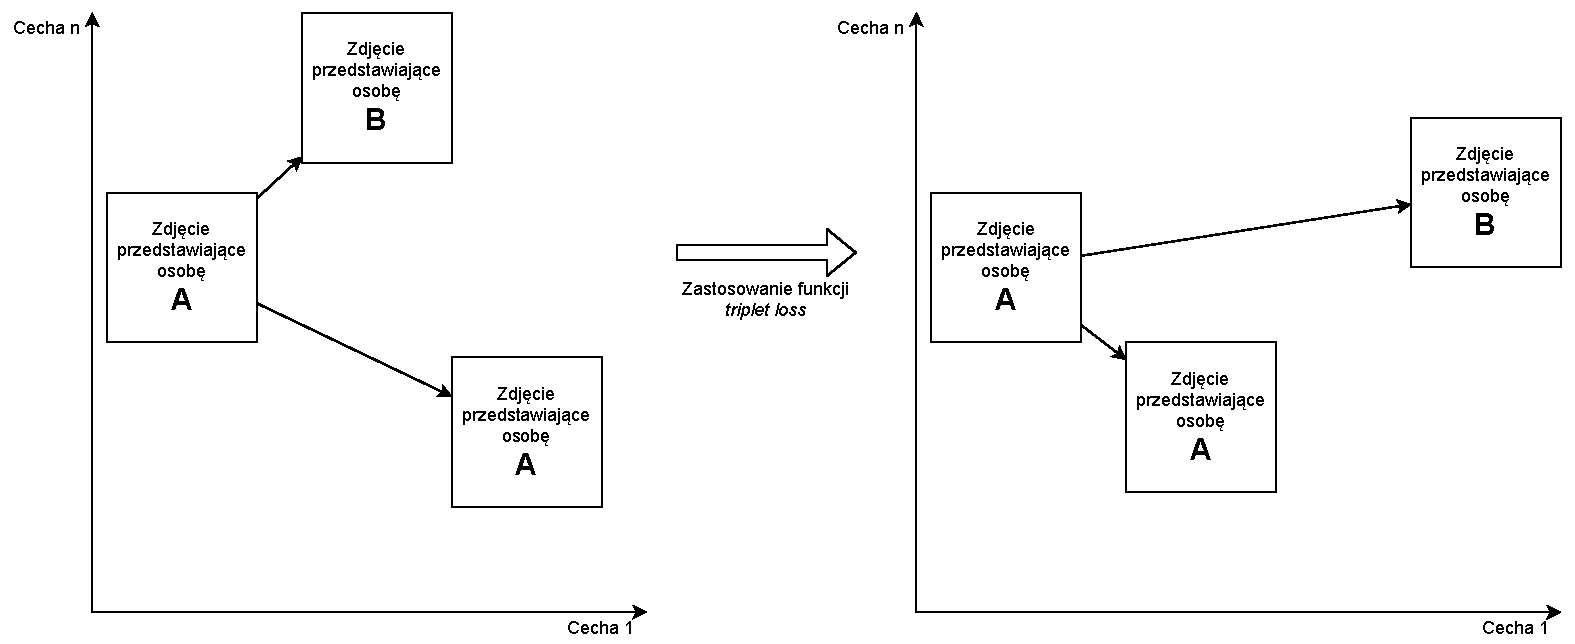
\includegraphics[width=1\textwidth]{images/triplet_loss}
    \caption{ Uproszczony schemat obrazujący zasadę działania funkcji strat \textit{triplet loss} }
    \customsource
    \label{fig:triplet_loss}
\end{figure}

Poszczególne etapy trenowania sieci o architekturze FaceNet zostały przedstawione na rysunku~\ref{fig:facenet_arch}.
Całość procesu uczenia się sieci FaceNet, można w uproszczeniu podsumować w następujących krokach:

\begin{enumerate}
    \item zdefiniowanie parametrów początkowych sieci,
    \item wygenerowanie wektorów cech twarzy,
    \item użycie funkcji strat \textit{triplet loss},
    \item dostosowanie się parametrów sieci tak, aby przykład pozytywny był bliżej zdjęcia wzorcowego, niż przykład negatywny,
    \item powrót do kroku drugiego tak długo, aż zwracane wektory osiągną zadaną dokładność.
\end{enumerate}

\bigskip
\bigskip

\begin{figure}[H]
    \centering
    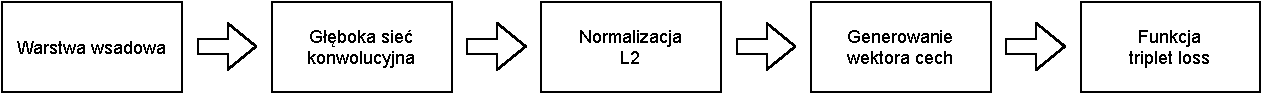
\includegraphics[width=1\textwidth]{images/facenet_arch}
    \caption{ Proces uczenia się sieci o architekturze FaceNet z podziałem na poszczególne etapy }
    \customsource
    \label{fig:facenet_arch}
\end{figure}

\subsection{Wpływ wielkości zdjęcia na działanie sieci}

W pracy pod tytułem \textit{Facenet: A unified embedding for face recognition and clustering}~\cite{schroff2015facenet}
została wytrenowana sieć o architekturze FaceNet na zdjęciach w formacie JPEG o rozmiarach 220 na 220 pikseli.
Podczas testowania wytrenowanej sieci, po dostarczeniu zdjęć o mniejszych rozmiarach (względem rozmiarów
zdjęć, na których sieć była trenowana) okazało się, że sieć ta jest również bardzo skuteczna.
Sieć miała akceptowalną skuteczność nawet po dostarczeniu zdjęć o rozmiarach 80 na 80 pikseli.
Trenowanie sieci na zdjęciach o mniejszej rozdzielczości mogłoby jeszcze poprawić ten wynik.
Dokładne informacje na temat wpływu liczby pikseli na
skuteczność sieci zostały przedstawione w tabeli~\ref{tab:quality_pixels_to_rate}

\begin{table}[H]
    \caption{
        Wpływ jakości zdjęcia oraz liczby pikseli na skuteczność sieci FaceNet.
        Źródło: \cite{schroff2015facenet}
    }
    \label{tab:quality_pixels_to_rate}
    \begin{minipage}{.5\linewidth}
        \centering
        \begin{tabular}{|l|l|}
            \hline
            Liczba pikseli                & Skuteczność \\ \hline
            1 600 \hspace{15px} (40x40)   & 37.8\%                \\ \hline
            6 400 \hspace{15px}     (80x80)    & 79.5\%                \\ \hline
            14 400 \hspace{10px}  (120x120) & 84.5\%                \\ \hline
            25 600 \hspace{10px}  (160x160) & 85.7\%                \\ \hline
            65 536 \hspace{10px}  (256x256) & 86.4\%                \\ \hline
        \end{tabular}
    \end{minipage}%
    \begin{minipage}{.5\linewidth}
        \centering
        \begin{tabular}{|l|l|}
            \hline
            Jakość JPEG & Skuteczność \\ \hline
            10          & 67.3\%      \\ \hline
            20          & 81.4\%      \\ \hline
            30          & 83.9\%      \\ \hline
            50          & 85.5\%      \\ \hline
            70          & 86.1\%      \\ \hline
            90          & 86.5\%      \\ \hline
        \end{tabular}
    \end{minipage}
\end{table}

\subsection{Użycie wytrenowanej sieci}

W projektowanym systemie zostanie użyty wytrenowany model \textit{Keras FaceNet}~\cite{taniai-2018},
który został wyszkolony na bazie zdjęć dostarczonych przez MS-Celeb-1M~\cite{microsoft-2020-celeb1m}
i udostępniony przez \textit{Hiroki Taniai}~\cite{taniai-no-date}.
Dostarczane zdjęcia twarzy powinny być kolorowe, w formacie RGB oraz
o rozmiarach 160 pikseli na 160 pikseli~\cite{brownlee-2019}.


\section{Kadrowanie i standaryzacja}

Do przetwarzania plików graficznych zostanie wykorzystana biblioteka \textit{PILLOW} napisana w języku python.
Biblioteka wspiera wiele formatów graficznych,
w tym te najpopularniejsze jak \textit{PNG}, \textit{GIF}, \textit{JPEG} oraz \textif{BMP}~\cite{pillow_doc},
dzięki czemu nie będzie wymagane, aby użytkownik sam konwertował plików graficznych do odpowiedniego formatu.
Biblioteka \textit{PILLOW} zostanie również wykorzystana do wycinania zdjęcia twarzy.

\pagebreak


\section{Klasyfikator SVM}

Ostatnim krokiem w systemie jest dokonanie klasyfikacji wygenerowanego wektora cech,
czyli określenie, do jakiej grupy należy wektor na podstawie próbek uczących.
Innymi słowy, etap ten polega na zwróceniu informacji, do kogo najbardziej pasuje przesłane zdjęcie,
opierając się na fotografiach dostępnych w systemie.

Jednym z szeroko stosowanych algorytmów klasyfikacji jest
\textbf{maszyna wektorów nośnych} (ang. support vector machine — SVM).
Klasyfikator ten konstruuje hiperpłaszczyznę lub ich zbiór w przestrzeni wielowymiarowej,
na podstawie otrzymanych próbek, która oddziela poszczególne klasy.
Optymalizowanie modelu SVM polega na maksymalizacji marginesu pomiędzy płaszczyzną a poszczególnymi klasami,
ponieważ na ogół nim większy margines, tym mniejszy jest błąd generalizacji~\cite{hastie2009elements}.
Koncepcja klasyfikatora została zaprezentowana na rysunku~\ref{fig:svm}.

\begin{figure}[H]
    \centering
    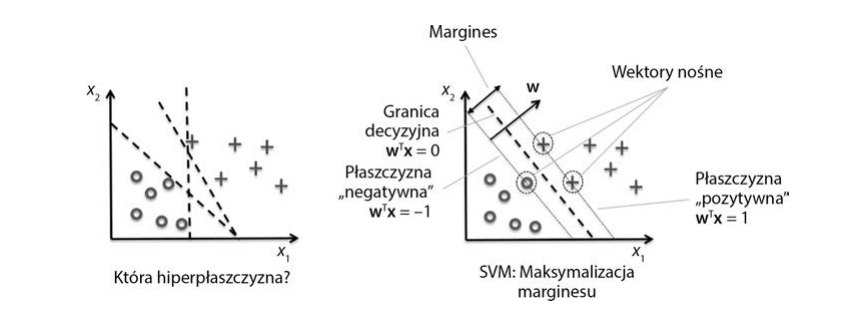
\includegraphics[width=1\textwidth]{images/smv}
    \caption{
        Model maszyny wektorów nośnych.
        Po lewej możliwe położenia hiperpłaszczyzny, po prawej zoptymalizowany model SVM.
    }
    \bibsource{\cite{raschka2017python}}
    \label{fig:svm}
\end{figure}

\pagebreak

\subsection{Margines twardy}

Jeśli dane uczące są liniowo separowalne, to można wybrać dwie równoległe hiperpłaszczyzny,
które oddzielają dwie klasy danych, tak aby odległość między nimi była maksymalna.
Obszar ograniczony przez te dwie hiperpłaszczyzny nazywany jest ``marginesem'',
a hiperpłaszczyzna maksymalnego marginesu to hiperpłaszczyzna leżąca w połowie odległości między nimi.
Problem optymalizacji algorytmu został przedstawiony równaniem~\ref{eq:hard_margin}~\cite{raschka2017python}.
Lewą stroną tego równania jest odległość pomiędzy hiperpłaszczyzną ``pozytywną'' a ``negatywną'',
zatem, w celu maksymalizacji marginesu, należy zmaksymalizować $\frac{2}{||w||}$ lub
minimalizować odwrotność wyrażenia, czyli $\frac{1}{2}||w||^2$.

\begin{equation}
    \begin{aligned}
        & \frac{ w^T (x_{poz} - x_{neg}) }{ ||w|| } = \frac{2}{||w||} \\
        \text{gdzie:} \\
        w & \text{ - wektor normalny do granicy decyzyjności}
        \\
        x_{poz} & \text{ - ``pozytywny'' wektor nośny}
        \\
        x_{neg} & \text{ - ``negatywny'' wektor nośny}
    \end{aligned}
    \label{eq:hard_margin}
\end{equation}
\bigskip

W przypadku danych liniowo separowalnych równanie~\ref{eq:hard_margin} musi
spełniać warunki przedstawione w równaniu~\ref{eq:hard_margin_class}~\cite{raschka2017python}.
Równania te oznaczają, że wszystkie negatywne próbki powinny wylądować po stronie
negatywnej hiperpłaszczyzny, a wszystkie próbki pozytywne po stronie hiperpłaszczyzny pozytywnej.

\begin{equation}
    \begin{aligned}
        w_0 +w^{T}x^{(i)} &\geq 1 && \text{ jeśli } y^{(i)} =1
        \\
        w_0 +w^{T}x^{(i)} &\leq -1 && \text{ jeśli } y^{(i)} =-1
        \\
        \text{dla } i&= 1\dots N
        \\
        \text{ gdzie: } \\
        N & \text{  - liczba próbek}
        \\
        w_0 +w^{T}x^{(i)} & \text{  - odległość od granicy decyzyjności}
    \end{aligned}
    \label{eq:hard_margin_class}
\end{equation}

\pagebreak

\subsection{Margines miękki}

W przypadku, gdy dane nie są liniowo separowalne (rysunek~\ref{fig:sofm_margin}) wprowadza się dodatkową zmienną $\xi$.
Motywacją wprowadzenia tej zmiennej jest potrzeba ``uelastycznienia'' liniowych
ograniczeń (równanie~\ref{eq:hard_margin_class}) podczas analizowania nieliniowo rozdzielnych danych,
co pozwala na uzyskanie zbieżności algorytmu uczącego w obecności nieprawidłowych klasyfikacji
podczas stosowania odpowiedniej funkcji strat.
Po wprowadzeniu zmiennej $\xi$ do równiania~\ref{eq:hard_margin_class},
równanie to przybiera postać opisaną wzorami~\ref{eq:soft_margin}~\cite{raschka2017python}.

\begin{equation}
    \begin{aligned}
        w_0 +w^{T}x^{(i)} &\geq 1 - \xi^{(i)} && \text{ jeśli } y^{(i)} =1
        \\
        w_0 +w^{T}x^{(i)} &\leq -1 + \xi^{(i)} && \text{ jeśli } y^{(i)} =-1
        \\
        \text{dla } i&= 1\dots N \\
        \text{gdzie:} \\
        N & \text{  - liczba próbek} \\
        \xi & \text{ - wartość przesunięcia granicy przynależności} \\
        w_0 +w^{T}x^{(i)} & \text{  - odległość od granicy decyzyjności}
    \end{aligned}
    \label{eq:soft_margin}
\end{equation}

\bigskip

\begin{figure}[H]
    \centering
    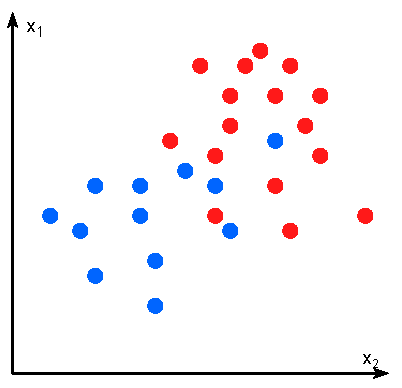
\includegraphics[width=0.4\textwidth]{images/soft-margin.drawio}
    \caption{ Przykład próbek nieliniowo rozdzielnych }
    \customsource
    \label{fig:sofm_margin}
\end{figure}

\pagebreak

\noindent Nowym celem optymalizacji staje wtedy się równanie~\ref{eq:hard_svm_min_problem}~\cite{raschka2017python}.
Za pomocą zmiennej $C$ kontroluje się wagę kary za niewłaściwą klasyfikację.
Duża wartość parametru $C$ odpowiada wysokim karom za błędy, z kolei przy niskich wartościach
kara nie będzie mocno wpływać na szerokość marginesu.
Dzięki temu parametrowi jest się w stanie regulować kompromis pomiędzy
obciążeniem a wariancją~\cite{raschka2017python} (rysunek~\ref{fig:wplyw_c_na_svm}).

\begin{equation}
    \begin{aligned}
        &\frac{1}{2}||w||^2 + C (\sum_{i}^{N} \xi^{(i)})\\
        \text{gdzie:} \\
        &C \text{ - mnożnik kary za złą klasyfikację}
    \end{aligned}
    \label{eq:hard_svm_min_problem}
\end{equation}

\bigskip
\bigskip
\bigskip

\begin{figure}[H]
    \centering
    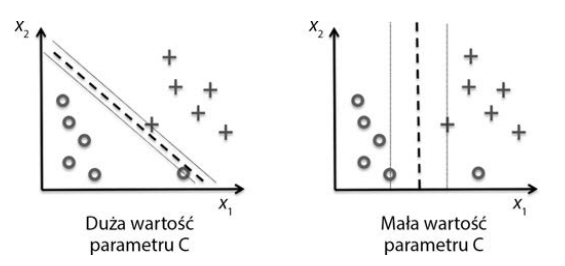
\includegraphics[width=0.7\textwidth]{images/wplyw_c_na_svm}
    \caption{  Wpływ zmiennej C na szerokość marginesu }
    \bibsource{\cite{raschka2017python}}
    \label{fig:wplyw_c_na_svm}
\end{figure}

\pagebreak

\subsection{Klasyfikacja nieliniowa}

W przypadku, gdy dostarczone dane nie są separowalne za pomocą hiperpłaszczyzny
w $N$ wymiarach (rysunek~\ref{fig:dane_nie_separowalne_liniowo})
wprowadza się dodatkowe wymiary za pomocą funkcji mapującej $\phi$.
Dodatkowe wymiary wprowadza się tak długo, aż dane staną się liniowo separowalne.
Przykładowo, w celu wyznaczenia granicy decyzyjności danych
przedstawionych na rysunku~\ref{fig:dane_nie_separowalne_liniowo},
funkcja mapująca, za pomocą której będzie możliwe wyznaczenie hiperpłaszczyzny,
została przedstawiona równaniem~\ref{eq:przykladowy_kernel}.
Rezultat mapowania danych z rysunku~\ref{fig:dane_nie_separowalne_liniowo} przez funkcję~\ref{eq:przykladowy_kernel}
został przedstawiony na rysunku~\ref{fig:wyniki_mapowan}.
Po wykonaniu mapowania oraz wyznaczeniu hiperpłaszczyzny dokonuje się rzutowania do pierwotnej przestrzeni cech ($\phi^{-1}$).

\begin{equation}
    \begin{aligned}
        \phi(x_1, x_2) = (z_1, z_2, z_3) = (x_1, x_2, x_1^2 + x_2^2)
    \end{aligned}
    \label{eq:przykladowy_kernel}
\end{equation}

\begin{figure}[H]
    \centering
    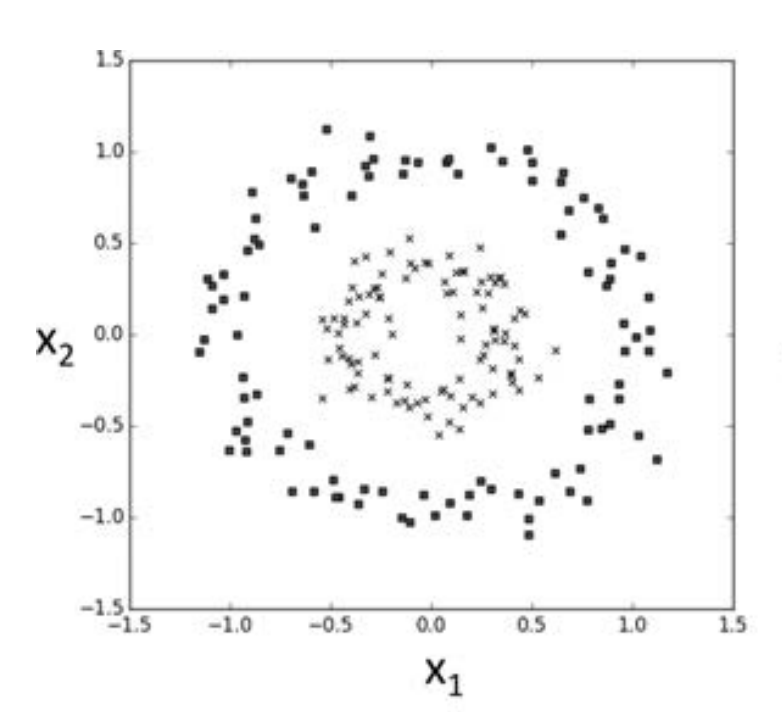
\includegraphics[width=0.3\textwidth]{images/dane_nie_separowalne_liniowo}
    \caption{  Zestaw danych nie separowalnych liniowo }
    \bibsource{\cite{raschka2017python}}
    \label{fig:dane_nie_separowalne_liniowo}
\end{figure}

\begin{figure}[H]
    \centering
    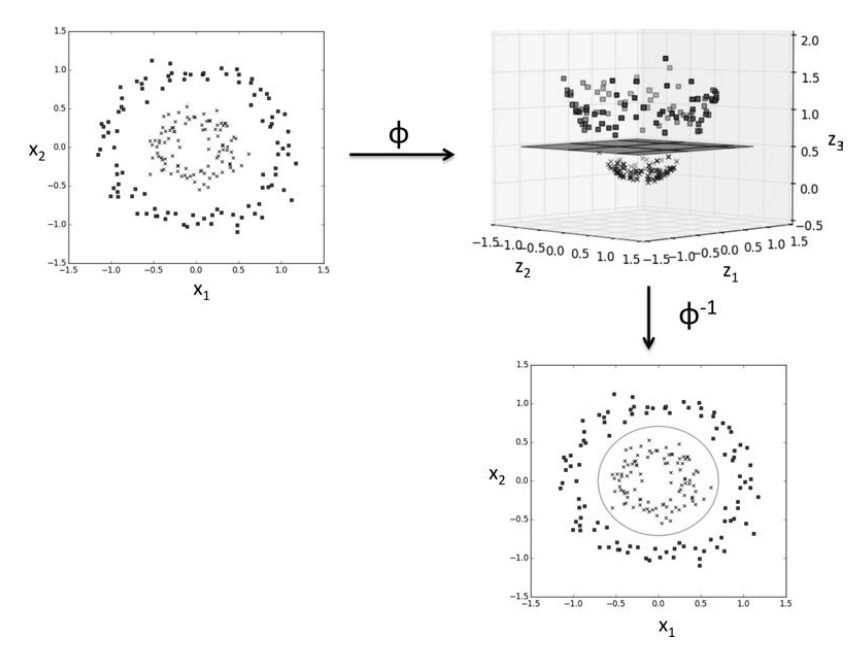
\includegraphics[width=1\textwidth]{images/wyniki_mapowan}
    \caption{ Sposób wyznaczania nieliniowej granicy decyzyjności }
    \bibsource{\cite{raschka2017python}}
    \label{fig:wyniki_mapowan}
\end{figure}

\pagebreak

\subsection{Klasyfikacja wieloklasowa}

Wszystkie opisane wyżej przypadki dotyczą problemów binarnych,
czyli takich gdzie dostarczona próbka należy do jednej z dwóch klas.
W związku z tym, że SVM obsługuje tylko klasyfikację binarną, dlatego w przypadku
gdy dana próbka może należeć do jeden z $N$ klas (klasyfikacja wieloklasowa)
dokonuje się rozbicia jednego problemu klasyfikacji wieloklasowej na wiele problemów klasyfikacji binarnej.
W tym celu stosuje się jedną z dwóch strategii - jeden kontra jeden (ang. one vs one --- OvO)
lub jeden przeciwko wszystkim (ang. one vs all --- OvA).
Obie te strategie zostały przedstawione na rysunku~\ref{fig:ovr} oraz~\ref{fig:ovo}.


\begin{figure}[H]
    \centering
    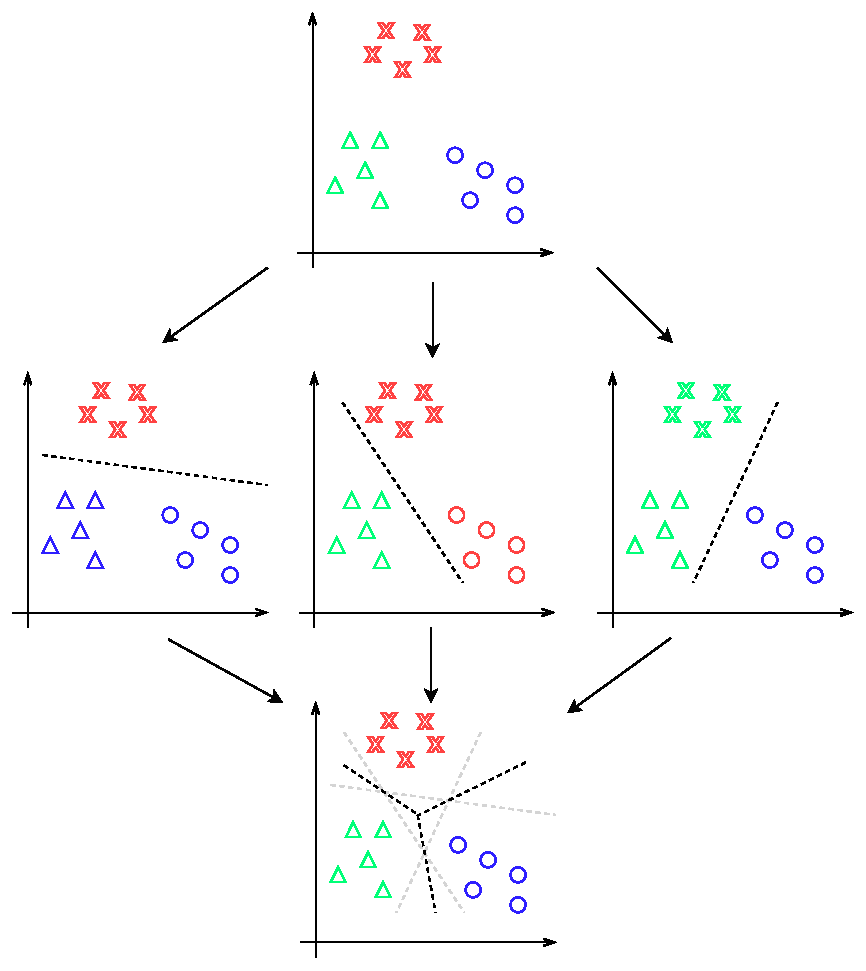
\includegraphics[width=0.7\textwidth]{images/ovr}
    \caption{ Strategia jeden przeciwko wszystkim }
    \customsource
    \label{fig:ovr}
\end{figure}

\begin{figure}[PH]
    \centering
    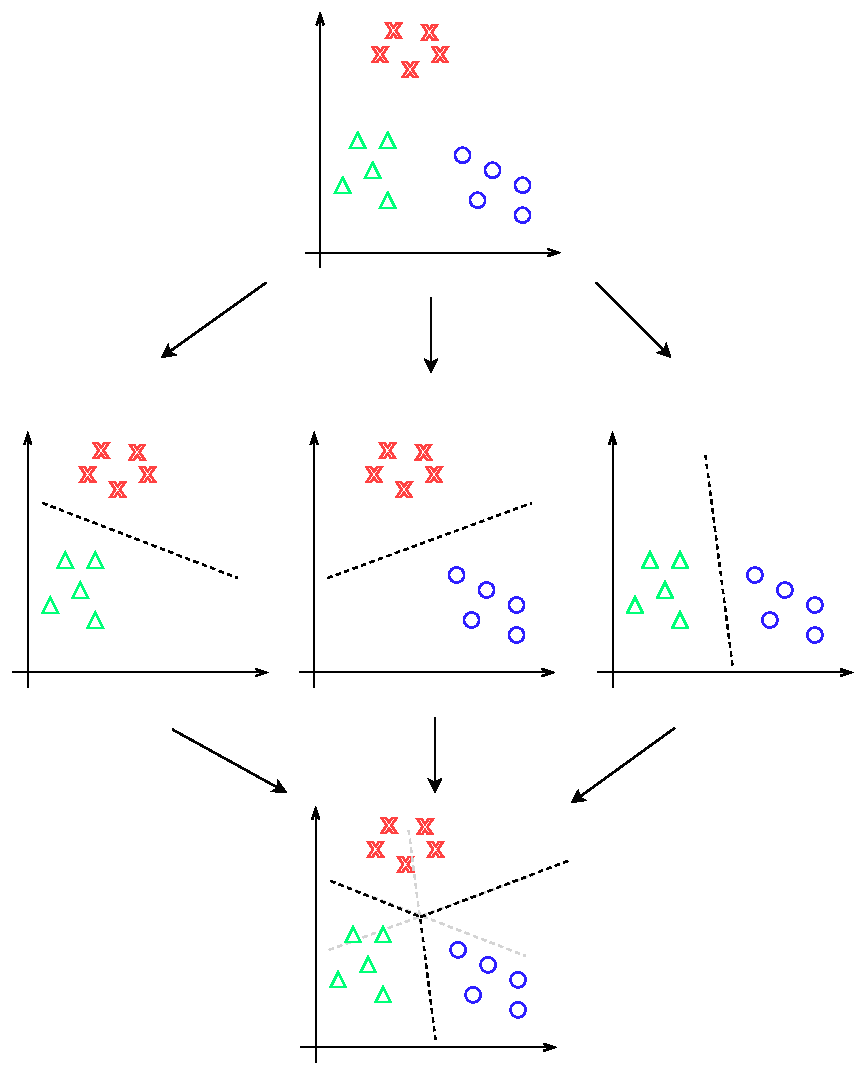
\includegraphics[width=0.7\textwidth]{images/ovo}
    \caption{ Strategia jeden kontra jeden }
    \customsource
    \label{fig:ovo}
\end{figure}

\pagebreak


\section{Obsługa systemu}

Całość zaprojektowanego systemu ma być dostępna z przeglądarki internetowej.
Aby sprostać temu wymaganiu, należy napisać usługę, która jest w stanie obsługiwać połączenia
HTTP (ang. Hypertext Transfer Protocol).
Z powodu, że narzędzia do wykrywania twarzy, obróbki zdjęć oraz FaceNet są udostępnione w języku python,
program zostanie również napisany w tym języku.
Oprócz samej strony internetowej potrzebna jest również baza danych,
w której będą przechowywane informacje o dostępnych zdjęciach.
Same zdjęcia będą przechowywane na serwerze plików.
Sporym ułatwieniem będzie również panel umożliwiający zarządzanie dostępnymi zdjęciami w systemie.

Narzędziem, które spełni wyżej postawione wymagania jest platforma programistyczna \textit{Django},
która umożliwia w łatwy sposób zarządzanie bazą danych za pomocą mapowania obiektowo-relacyjnego,
pozwala na zarządzanie danymi dostępnymi w bazie danych poprzez panel administratora, dostępny
z poziomu przeglądarki oraz co najważniejsze, jest napisana w języku python~\cite{djangodoc}.